\documentclass[11pt,psfig]{article}
\usepackage{epsfig}
\usepackage{times}
\usepackage{amssymb}
\usepackage{float}

\newcount\refno\refno=1
\def\ref{\the\refno \global\advance\refno by 1}
\def\ux{\underline{x}}
\def\uw{\underline{w}}
\def\bw{\underline{w}}
\def\ut{\underline{\theta}}
\def\umu{\underline{\mu}} 
\def\bmu{\underline{\mu}} 
\def\be{p_e^*}
\newcount\eqnumber\eqnumber=1
\def\eq{\the \eqnumber \global\advance\eqnumber by 1}
\def\eqs{\eq}
\def\eqn{\eqno(\eq)}

 \pagestyle{empty}
\def\baselinestretch{1.1}
\topmargin1in \headsep0.3in
\topmargin0in \oddsidemargin0in \textwidth6.5in \textheight8.5in
\begin{document}
\setlength{\parskip}{1.2ex plus0.3ex minus 0.3ex}


\thispagestyle{empty} \pagestyle{myheadings} \markright{Homework
1: CS 273, Machine Learning: Winter 2015}



\title{CS 273 Homework 1}
\author{Zachary DeStefano, 15247592}
\date{Due Date: Tuesday, January 13, 2015}

\maketitle

\vfill\eject

%\begin{figure}[H]
%\centering
%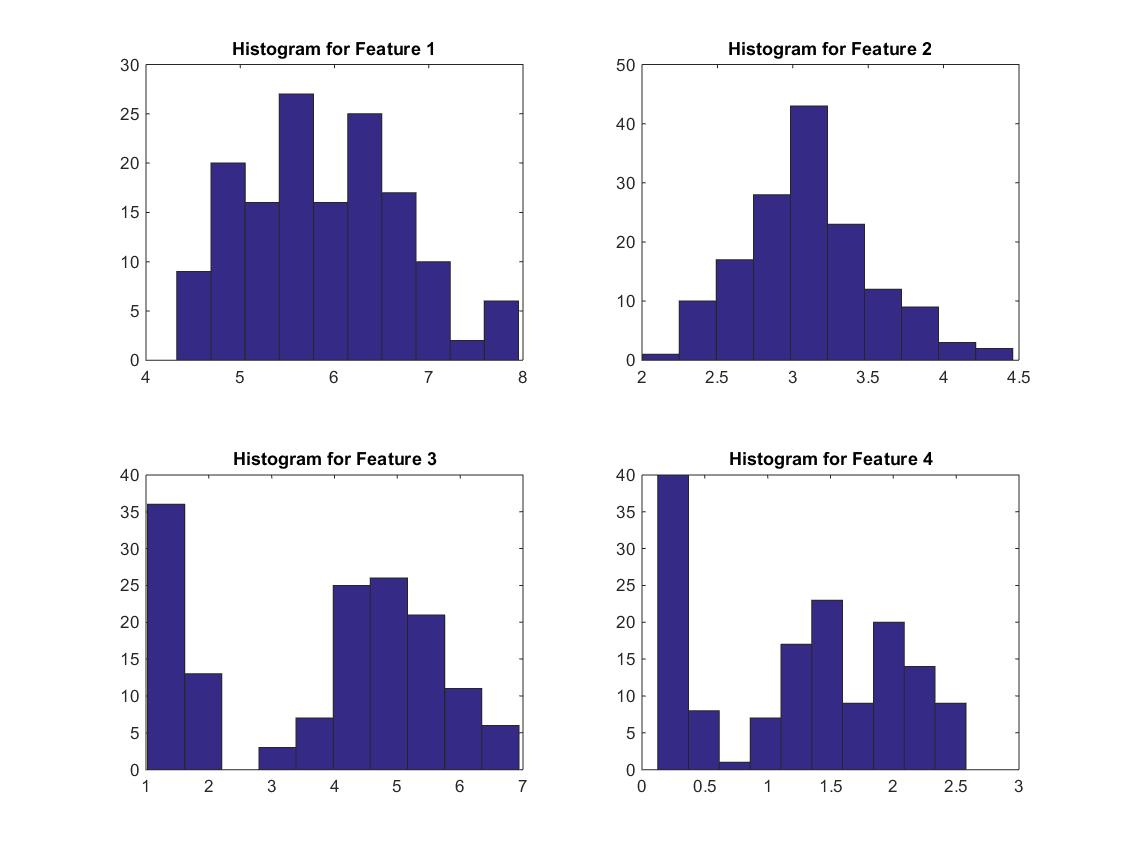
\includegraphics[width=\columnwidth]{prob1bHistograms.jpg}
%\caption{Histograms for each feature}
%\end{figure}

\section*{Problem 1}

\subsection*{Problem 1, Part a}

The number of features is 4\\
The number of observations is 148\\

\subsection*{Problem 1, Part b}

\begin{figure}[H]
\centering
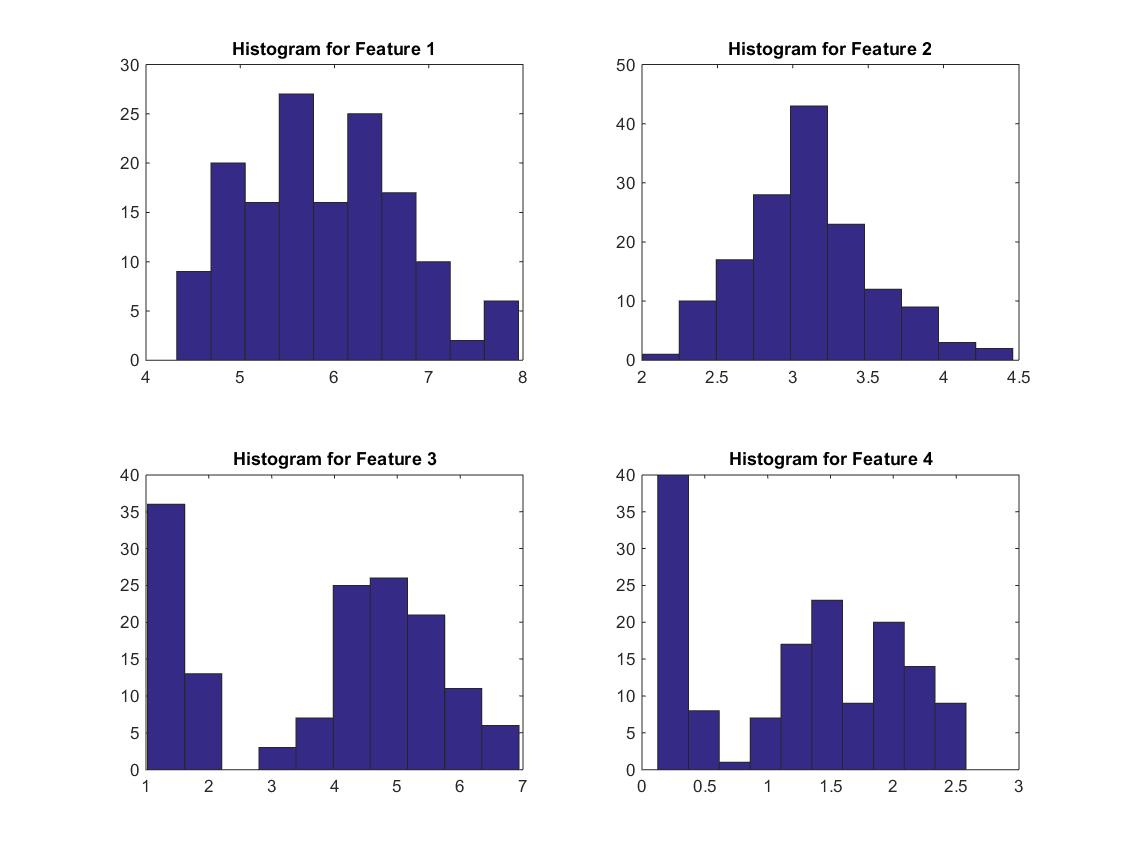
\includegraphics[width=\columnwidth]{prob1bHistograms.jpg}
\caption{Histograms for each feature}
\end{figure}

\newpage

\subsection*{Problem 1, Part c}

The mean of feature 1 is 5.9001\\
The mean of feature 2 is 3.0989\\
The mean of feature 3 is 3.8196\\
The mean of feature 4 is 1.2526\\

\subsection*{Problem 1, Part d}

The variance of feature 1 is 0.6993\\
The variance of feature 2 is 0.1916\\
The variance of feature 3 is 3.0976\\
The variance of feature 4 is 0.5797\\
\\
The standard deviation of feature 1 is 0.8362\\
The standard deviation of feature 2 is 0.4378\\
The standard deviation of feature 3 is 1.7600\\
The standard deviation of feature 4 is 0.7613\\

\subsection*{Problem 1, Part e}

Here is the code for part E. The initial parts of the code covers previous parts of this problem. 
\begin{verbatim}
iris = load('data/iris.txt');
y = iris(:,end);
X = iris(:,1:end-1);

%part A
numFeatures = size(X,2);
numDataPoints = size(X,1);

%put features into vectors
feature1 = X(:,1);
feature2 = X(:,2);
feature3 = X(:,3);
feature4 = X(:,4);

%part B
figure
subplot(2,2,1)
hist(feature1)
title('Histogram for Feature 1')
subplot(2,2,2)
hist(feature2)
title('Histogram for Feature 2')
subplot(2,2,3)
hist(feature3)
title('Histogram for Feature 3')
subplot(2,2,4)
hist(feature4)
title('Histogram for Feature 4')

%part C
mean1 = mean(feature1);
mean2 = mean(feature2);
mean3 = mean(feature3);
mean4 = mean(feature4);


%part D

%compute the variance
var1 = var(feature1);
var2 = var(feature2);
var3 = var(feature3);
var4 = var(feature4);

%compute the standard deviation
std1 = std(feature1);
std2 = std(feature2);
std3 = std(feature3);
std4 = std(feature4);

%part E
% Normalizes the data
normalize1 = (feature1-mean1)/std1;
normalize2 = (feature2-mean2)/std2;
normalize3 = (feature3-mean3)/std3;
normalize4 = (feature4-mean4)/std4;

\end{verbatim}

\subsection*{Problem 1, Part f}

\begin{figure}[H]
\centering
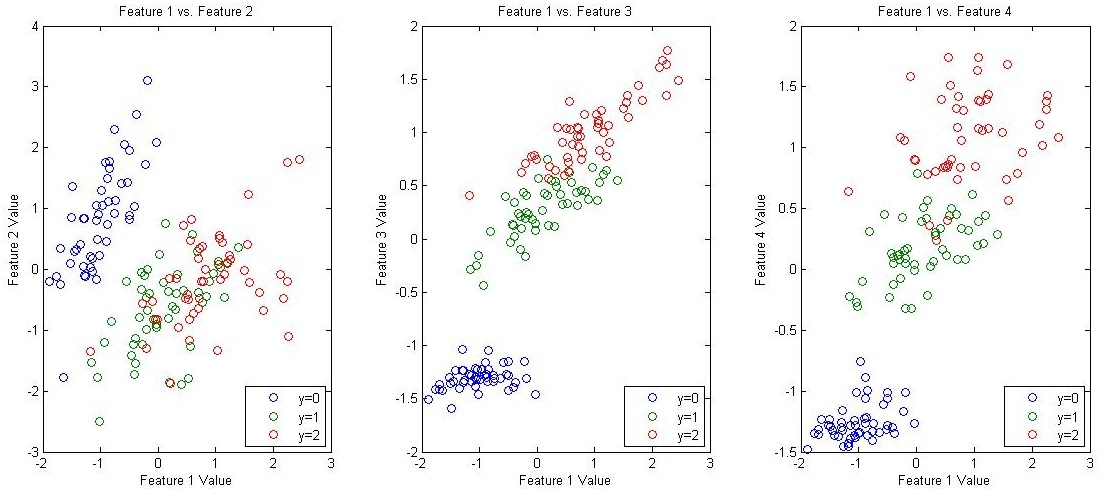
\includegraphics[width=\columnwidth]{prob1fScatterPlots.jpg}
\caption{The scatter plots for Problem 1f}
\end{figure}

This is the code to make those plots. It is a continuation of the code posted for part e. 
\begin{verbatim}
size = 30;
figure
subplot(1,3,1)
scatter(normalize1,normalize2,size,y);
title('Feature 1 vs. Feature 2');
xlabel('Feature 1 Value');
ylabel('Feature 2 Value');
subplot(1,3,2)
scatter(normalize1,normalize3,size,y);
title('Feature 1 vs. Feature 3');
xlabel('Feature 1 Value');
ylabel('Feature 3 Value');
subplot(1,3,3)
scatter(normalize1,normalize4,size,y);
title('Feature 1 vs. Feature 4');
xlabel('Feature 1 Value');
ylabel('Feature 4 Value');
\end{verbatim}

\newpage

\section*{Problem 2}

\subsection*{Problem 2, Part a}

These are the plots for part a

\begin{figure}[H]
\centering
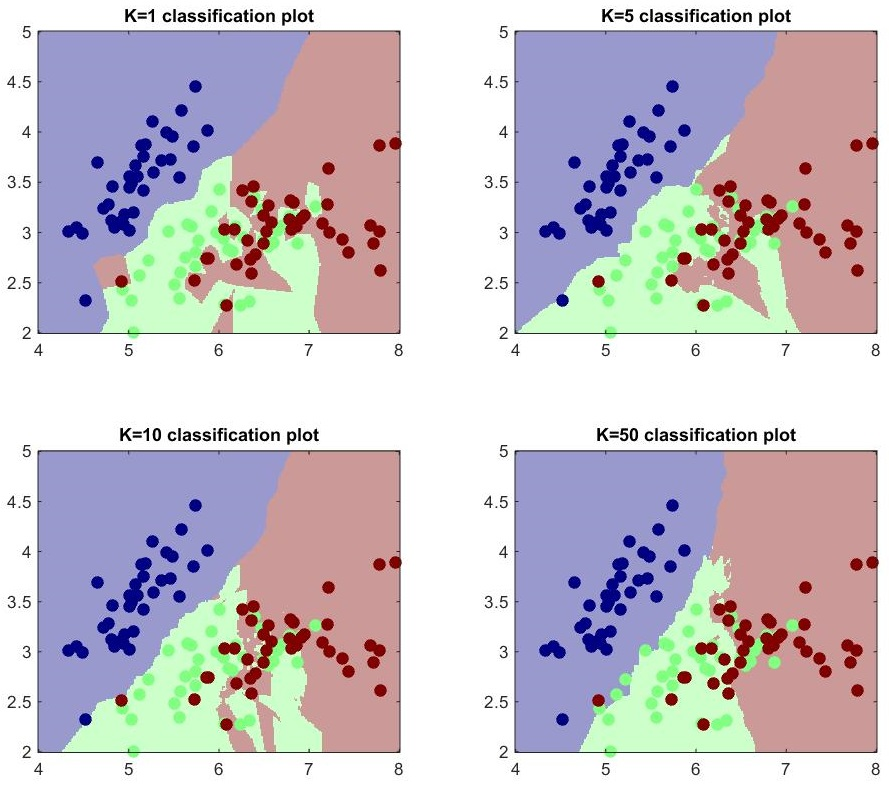
\includegraphics[width=\columnwidth]{prob2aPlots.jpg}
\caption{The scatter plots for Problem 2a}
\end{figure}

\newpage

Here is the code I used to generate those plots

\begin{verbatim}
%InitialPart
iris=load('data/iris.txt'); 
y=iris(:,end); 
X=iris(:,1:end-1);

[X y] = shuffleData(X,y); % shuffle data randomly
[Xtr Xte Ytr Yte] = splitData(X,y, .75); % split data into 75/25 train/test

%gets the first 2 features
XtrFirstTwo = Xtr(:,1:2);
XteFirstTwo = Xte(:,1:2);

%partA
figure
Kvals = [1,5,10,50];
for i=1:4
   K = Kvals(i);
   
   %train the classifier
   knn = knnClassify( XtrFirstTwo, Ytr, K );
   
   % make 2D classification plot
   subplot(2,2,i)
   plotClassify2D( knn, XtrFirstTwo, Ytr );
   title(strcat('K=',num2str(K),' classification plot'));
end
\end{verbatim}

\newpage

\subsection*{Problem 2, Part b}

Here is the training error (in Red) and the test error (in green) as the value of K increases. \\
Based on this plot, I would recommend $K=50$

\begin{figure}[H]
\centering
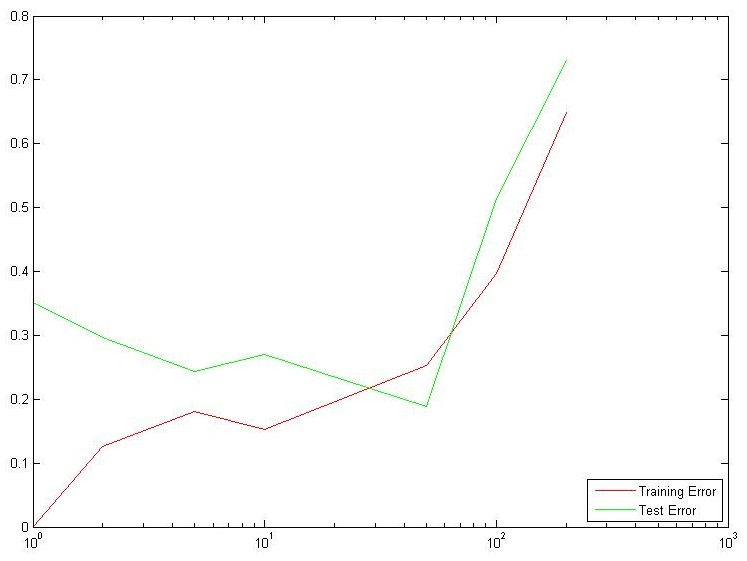
\includegraphics[width=\columnwidth]{prob2bPlot.jpg}
\caption{The semilog plot for Problem 2}
\end{figure}

\newpage

This is the rest of the code for problem 2, the part which was used to make the plots for part b. 

\begin{verbatim}
%part B
Kvals=[1,2,5,10,50,100,200];
errTrain=zeros(1,length(Kvals));
errTest = zeros(1,length(Kvals));
for i=1:length(Kvals)
    K = Kvals(i);
    learner = knnClassify( XtrFirstTwo, Ytr, K );
    YhatTr = predict(learner,XtrFirstTwo);
    errTrain(i)=length(find(YhatTr~=Ytr))/length(Ytr);
    
    YhatTe = predict(learner,XteFirstTwo);
    errTest(i)=length(find(YhatTe~=Yte))/length(Yte);
end;
figure
hold on
semilogx(Kvals,errTrain,'-','LineWidth',2,'Color','red');
semilogx(Kvals,errTest,'-','LineWidth',2,'Color','green');
hold off
\end{verbatim}

\newpage

\section*{Problem 3}

\subsection*{Problem 3, Part a}

The class probabilities are as follows:\\
$p(y=1) = 0.4$\\
$p(y=-1) = 0.6$\\
\\
The feature probabilites are as follows:\\
\begin{tabular}{ l | c | c | c | c}
  i   & $p(x_i=0|y=1)$ & $p(x_i=1|y=1)$ & $p(x_i=0|y=1)$ & $p(x_i=1|y=1)$\\
\hline
  1 & 0.25 & 0.75 & 0.5 & 0.5 \\
  2 & 1&0 & 0.1667 & 0.8333\\
  3 & 0.25 & 0.75 & 0.3333 & 0.6667\\
  4 & 0.5 & 0.5 & 0.1667 & 0.8333\\
  5 & 0.75 & 0.25 & 0.6667 & 0.3333\\
\end{tabular}
\\
\\
\\
Here is the code I used to get those values

\begin{verbatim}
xyData=[
0 0 1 1 0 -1;
1 1 0 1 0 -1;
0 1 1 1 1 -1;
1 1 1 1 0 -1;
0 1 0 0 0 -1;
1 0 1 1 1 1;
0 0 1 0 0 1;
1 0 0 0 0 1;
1 0 1 1 0 1;
1 1 1 1 1 -1];   

X=xyData(:,1:5);
y=xyData(:,6);

%Part A

%this gets p(y==1) and p(y==-1)
indicesY1 = find(y==1);
indicesYminus1 = find(y==-1);
probY1 = length(indicesY1)/length(y);
probYminus1 = 1-probY1;

%in order to get class probabilities, we go over entries where
%       y==1 and y==-1
%
% We will get the following matrices
%   probXwhereY1:
%       row i has probabilities for x_i
%       column 1 is p(x_i=0|y=1)
%       column 2 is p(x_i=1|y=1)
%   probXwhereYminus1:
%       row i has probabilities for x_i
%       column 1 is p(x_i=0|y=-1)
%       column 2 is p(x_i=1|y=-1)
probXwhereY1 = zeros(5,2);
probXwhereYminus1 = zeros(5,2);
for i = 1:5
    Xi = X(:,i);
    
    XiwhereY1 = Xi(indicesY1); %x_i values for entries where y=1
    probXwhereY1(i,1) = length(find(XiwhereY1==0))/length(XiwhereY1);
    probXwhereY1(i,2) = 1-probXwhereY1(i,1);
    
    XiwhereYminus1 = Xi(indicesYminus1); %x_i values for entries where y=-1
    probXwhereYminus1(i,1) = length(find(XiwhereYminus1==0))/length(XiwhereYminus1);
    probXwhereYminus1(i,2) = 1-probXwhereYminus1(i,1);
end
\end{verbatim}

\subsection*{Problem 3, Part b}

With $x=(0,0,0,0,0)$ it holds that \\
$p(y=1)=0.8351$\\
$p(y=-1)=0.1649$\\
Thus $y=1$ is the predicted classification.\\
\\
With $x=(1,1,0,1,0)$ it holds that \\
$p(y=1)=0$ \\
$p(y=-1)=1$ \\
Thus $y=-1$ is the predicted classification.\\

\subsection*{Problem 3, Part c}

The values showed in my answer for part b are the normalized values, thus \\
$p(y=1)=0$ for $x=(1,1,0,1,0)$ as noted previously.

\subsection*{Problem 3, Part b and c code}

Here is the code that I used to compute the values in part b and c. \\
This is a continuation of the code from part a.

\begin{verbatim}
%part B
%Using Naive Bayes, p(y|x) = p(x|y)p(y)/p(x)
%   p(x) = sum_y( p(x|y)p(y) )
%   p(x|y)=p(x_1|y)p(x_2|y)...p(x_5|y)

%We need to find the y prob of x=(0 0 0 0 0)
xTest1 = [0 0 0 0 0];
[probY1withXtest1,probYminus1withXtest1] = prob3Classifier(probXwhereY1,probXwhereYminus1,probY1,probYminus1,xTest1);

bestYclassification1 = 1;
if(probY1withXtest1<probYminus1withXtest1)
    bestYclassification1 = -1; 
end

xTest2 = [1 1 0 1 0];
[probY1withXtest2,probYminus1withXtest2] = prob3Classifier(probXwhereY1,probXwhereYminus1,probY1,probYminus1,xTest2);

bestYclassification2 = 1;
if(probY1withXtest2<probYminus1withXtest2)
    bestYclassification2 = -1; 
end

%part C
probY1withXtest2
\end{verbatim}

\newpage

I wrote a function called {\it prob3Classifier} that used the classifier made in part a \\
and computed the posterior probabilities. Here is the code for it:

\begin{verbatim}
function [ probY1withXtest1,probYminus1withXtest1 ] = prob3Classifier( 
probXwhereY1,probXwhereYminus1, probY1, probYminus1,xTest1 )
%PROB3CLASSIFIER says the probabilities of the classifications of the test
%               data
% Input is the following matrices:
%   probXwhereY1:
%       row i has probabilities for x_i
%       column 1 is p(x_i=0|y=1)
%       column 2 is p(x_i=1|y=1)
%   probXwhereYminus1:
%       row i has probabilities for x_i
%       column 1 is p(x_i=0|y=-1)
%       column 2 is p(x_i=1|y=-1)
%
%probY1withXtest1 is p(y=1|x) where x is the test vector
%probYminus1withXtest1 is p(y=-1|x) where x is the test vector

probXtestWhereY1 = zeros(1,5);
probXtestWhereYminus1 = zeros(1,5);
for i = 1:5
   probXtestWhereY1(i) = probXwhereY1(i,xTest1(i)+1); 
   probXtestWhereYminus1(i) = probXwhereYminus1(i,xTest1(i)+1); 
end
probXtestWithY1 = prod(probXtestWhereY1)*probY1;
probXtestWithYminus1 = prod(probXtestWhereYminus1)*probYminus1;

%finally here is p(y=1|x)
probY1withXtest1 = probXtestWithY1/(probXtestWithY1+probXtestWithYminus1);

%here is p(y=-1|x)
probYminus1withXtest1 = probXtestWithYminus1/(probXtestWithY1+probXtestWithYminus1);

end
\end{verbatim}

\newpage

\subsection*{Problem 3, part d}

We have 5 features with 2 values each, so if we want a Bayes classifier then there are $2^5=32$ feature vectors which we would need to find classification probabilities for. We only have 10 observations meaning that not all the feature vectors have a classification probability. We thus would not have a trained Bayes classifier and there could be input values that it could not compute a probability for.\\
\\
Another issue with using a Bayes classifier is that each row is unique so the probability for each class given a feature vector would simply be 0 or 1 which is likely not accurate.

\newpage

\section*{Problem 4}

\subsection*{Problem 4, Part a}
The mean vectors for the first two features are as follows:\\
\\
For class $y=0$ it is the following: $(5.0094,3.4460)$\\
For class $y=1$ it is the following: $(5.9934,2.7838)$\\
For class $y=2$ it is the following: $(6.5927,3.0392)$\\
\\
\\
The covariance matrices for the first two features are as follows:\\
\\
For class $y=0$ it is the following:\\
\begin{tabular}{l c}
0.1239 & 0.1038\\
0.1038 & 0.1542\\
\end{tabular}
\\
\\
For class $y=1$ it is the following:\\
\begin{tabular}{l c}
0.2781 & 0.0921\\
0.0921 & 0.1008\\
\end{tabular}
\\
\\
For class $y=2$ it is the following:\\
\begin{tabular}{l c}
0.3956 & 0.1377\\
0.1377 & 0.1277\\
\end{tabular}
\\

\end{document}








